\documentclass[a4paper,12pt,twoside]{memoir}

% Castellano
\usepackage[spanish,es-tabla]{babel}
\selectlanguage{spanish}
\usepackage[utf8]{inputenc}
\usepackage[T1]{fontenc}
\usepackage{lmodern} % Scalable font
\usepackage{microtype}
\usepackage{placeins}

\RequirePackage{booktabs}
\RequirePackage[table]{xcolor}
\RequirePackage{xtab}
\RequirePackage{multirow}

% Links
\PassOptionsToPackage{hyphens}{url}\usepackage[colorlinks]{hyperref}
\hypersetup{
	allcolors = {red}
}

% Ecuaciones
\usepackage{amsmath}

% Rutas de fichero / paquete
\newcommand{\ruta}[1]{{\sffamily #1}}

% Párrafos
\nonzeroparskip

% Huérfanas y viudas
\widowpenalty100000
\clubpenalty100000

% Imágenes

% Comando para insertar una imagen en un lugar concreto.
% Los parámetros son:
% 1 --> Ruta absoluta/relativa de la figura
% 2 --> Texto a pie de figura
% 3 --> Tamaño en tanto por uno relativo al ancho de página
\usepackage{graphicx}
\newcommand{\imagen}[3]{
	\begin{figure}[!h]
		\centering
		\includegraphics[width=#3\textwidth]{#1}
		\caption{#2}\label{fig:#1}
	\end{figure}
	\FloatBarrier
}

% Comando para insertar una imagen sin posición.
% Los parámetros son:
% 1 --> Ruta absoluta/relativa de la figura
% 2 --> Texto a pie de figura
% 3 --> Tamaño en tanto por uno relativo al ancho de página
\newcommand{\imagenflotante}[3]{
	\begin{figure}
		\centering
		\includegraphics[width=#3\textwidth]{#1}
		\caption{#2}\label{fig:#1}
	\end{figure}
}

% El comando \figura nos permite insertar figuras comodamente, y utilizando
% siempre el mismo formato. Los parametros son:
% 1 --> Porcentaje del ancho de página que ocupará la figura (de 0 a 1)
% 2 --> Fichero de la imagen
% 3 --> Texto a pie de imagen
% 4 --> Etiqueta (label) para referencias
% 5 --> Opciones que queramos pasarle al \includegraphics
% 6 --> Opciones de posicionamiento a pasarle a \begin{figure}
\newcommand{\figuraConPosicion}[6]{%
  \setlength{\anchoFloat}{#1\textwidth}%
  \addtolength{\anchoFloat}{-4\fboxsep}%
  \setlength{\anchoFigura}{\anchoFloat}%
  \begin{figure}[#6]
    \begin{center}%
      \Ovalbox{%
        \begin{minipage}{\anchoFloat}%
          \begin{center}%
            \includegraphics[width=\anchoFigura,#5]{#2}%
            \caption{#3}%
            \label{#4}%
          \end{center}%
        \end{minipage}
      }%
    \end{center}%
  \end{figure}%
}

%
% Comando para incluir imágenes en formato apaisado (sin marco).
\newcommand{\figuraApaisadaSinMarco}[5]{%
  \begin{figure}%
    \begin{center}%
    \includegraphics[angle=90,height=#1\textheight,#5]{#2}%
    \caption{#3}%
    \label{#4}%
    \end{center}%
  \end{figure}%
}
% Para las tablas
\newcommand{\otoprule}{\midrule [\heavyrulewidth]}
%
% Nuevo comando para tablas pequeñas (menos de una página).
\newcommand{\tablaSmall}[5]{%
 \begin{table}
  \begin{center}
   \rowcolors {2}{gray!35}{}
   \begin{tabular}{#2}
    \toprule
    #4
    \otoprule
    #5
    \bottomrule
   \end{tabular}
   \caption{#1}
   \label{tabla:#3}
  \end{center}
 \end{table}
}

%
% Nuevo comando para tablas pequeñas (menos de una página).
\newcommand{\tablaSmallSinColores}[5]{%
 \begin{table}[H]
  \begin{center}
   \begin{tabular}{#2}
    \toprule
    #4
    \otoprule
    #5
    \bottomrule
   \end{tabular}
   \caption{#1}
   \label{tabla:#3}
  \end{center}
 \end{table}
}

\newcommand{\tablaApaisadaSmall}[5]{%
\begin{landscape}
  \begin{table}
   \begin{center}
    \rowcolors {2}{gray!35}{}
    \begin{tabular}{#2}
     \toprule
     #4
     \otoprule
     #5
     \bottomrule
    \end{tabular}
    \caption{#1}
    \label{tabla:#3}
   \end{center}
  \end{table}
\end{landscape}
}

%
% Nuevo comando para tablas grandes con cabecera y filas alternas coloreadas en gris.
\newcommand{\tabla}[6]{%
  \begin{center}
    \tablefirsthead{
      \toprule
      #5
      \otoprule
    }
    \tablehead{
      \multicolumn{#3}{l}{\small\sl continúa desde la página anterior}\\
      \toprule
      #5
      \otoprule
    }
    \tabletail{
      \hline
      \multicolumn{#3}{r}{\small\sl continúa en la página siguiente}\\
    }
    \tablelasttail{
      \hline
    }
    \bottomcaption{#1}
    \rowcolors {2}{gray!35}{}
    \begin{xtabular}{#2}
      #6
      \bottomrule
    \end{xtabular}
    \label{tabla:#4}
  \end{center}
}

%
% Nuevo comando para tablas grandes con cabecera.
\newcommand{\tablaSinColores}[6]{%
  \begin{center}
    \tablefirsthead{
      \toprule
      #5
      \otoprule
    }
    \tablehead{
      \multicolumn{#3}{l}{\small\sl continúa desde la página anterior}\\
      \toprule
      #5
      \otoprule
    }
    \tabletail{
      \hline
      \multicolumn{#3}{r}{\small\sl continúa en la página siguiente}\\
    }
    \tablelasttail{
      \hline
    }
    \bottomcaption{#1}
    \begin{xtabular}{#2}
      #6
      \bottomrule
    \end{xtabular}
    \label{tabla:#4}
  \end{center}
}

%
% Nuevo comando para tablas grandes sin cabecera.
\newcommand{\tablaSinCabecera}[5]{%
  \begin{center}
    \tablefirsthead{
      \toprule
    }
    \tablehead{
      \multicolumn{#3}{l}{\small\sl continúa desde la página anterior}\\
      \hline
    }
    \tabletail{
      \hline
      \multicolumn{#3}{r}{\small\sl continúa en la página siguiente}\\
    }
    \tablelasttail{
      \hline
    }
    \bottomcaption{#1}
  \begin{xtabular}{#2}
    #5
   \bottomrule
  \end{xtabular}
  \label{tabla:#4}
  \end{center}
}



\definecolor{cgoLight}{HTML}{EEEEEE}
\definecolor{cgoExtralight}{HTML}{FFFFFF}

%
% Nuevo comando para tablas grandes sin cabecera.
\newcommand{\tablaSinCabeceraConBandas}[5]{%
  \begin{center}
    \tablefirsthead{
      \toprule
    }
    \tablehead{
      \multicolumn{#3}{l}{\small\sl continúa desde la página anterior}\\
      \hline
    }
    \tabletail{
      \hline
      \multicolumn{#3}{r}{\small\sl continúa en la página siguiente}\\
    }
    \tablelasttail{
      \hline
    }
    \bottomcaption{#1}
    \rowcolors[]{1}{cgoExtralight}{cgoLight}

  \begin{xtabular}{#2}
    #5
   \bottomrule
  \end{xtabular}
  \label{tabla:#4}
  \end{center}
}



\graphicspath{ {./img/} }

% Capítulos
\chapterstyle{bianchi}
\newcommand{\capitulo}[2]{
	\setcounter{chapter}{#1}
	\setcounter{section}{0}
	\setcounter{figure}{0}
	\setcounter{table}{0}
	\chapter*{#2}
	\addcontentsline{toc}{chapter}{#2}
	\markboth{#2}{#2}
}

% Apéndices
\renewcommand{\appendixname}{Apéndice}
\renewcommand*\cftappendixname{\appendixname}

\newcommand{\apendice}[1]{
	%\renewcommand{\thechapter}{A}
	\chapter{#1}
}

\renewcommand*\cftappendixname{\appendixname\ }

% Formato de portada
\makeatletter
\usepackage{xcolor}
\newcommand{\tutor}[1]{\def\@tutor{#1}}
\newcommand{\course}[1]{\def\@course{#1}}
\definecolor{cpardoBox}{HTML}{E6E6FF}
\def\maketitle{
  \null
  \thispagestyle{empty}
  % Cabecera ----------------
\noindent
\includegraphics[width=\textwidth]{cabecera}\vspace{1cm}%
  \vfill
  % Título proyecto y escudo informática ----------------
  \colorbox{cpardoBox}{%
    \begin{minipage}{.8\textwidth}
      \vspace{.5cm}\Large
      \begin{center}
      \textbf{TFG del Grado en Ingeniería Informática}\vspace{.6cm}\\
      \textbf{\LARGE\@title{}}
      \end{center}
      \vspace{.2cm}
    \end{minipage}

  }%
  \hfill\begin{minipage}{.20\textwidth}
    
\includegraphics[width=\textwidth]{escudoInfor}
  \end{minipage}
  \vfill
  % Datos de alumno, curso y tutores ------------------
  \begin{center}%
  {%
    \noindent\LARGE
    Presentado por \@author{}\\ 
    en Universidad de Burgos --- \@date{}\\
    Tutor: \@tutor{}\\
  }%
  \end{center}%
  \null
  \cleardoublepage
  }
\makeatother

\newcommand{\nombre}{Nombre del alumno} %%% cambio de comando

% Datos de portada
\title{XacoMeter II}
\author{Natalia Franco Peciña}
\tutor{Jose Ignacio Santos Martín, Virginia Ahedo García y Silvia Díaz de la Fuente}
\date{\today}

\begin{document}

\maketitle


\newpage\null\thispagestyle{empty}\newpage


%%%%%%%%%%%%%%%%%%%%%%%%%%%%%%%%%%%%%%%%%%%%%%%%%%%%%%%%%%%%%%%%%%%%%%%%%%%%%%%%%%%%%%%%
\thispagestyle{empty}


\noindent
\includegraphics[width=\textwidth]{cabecera}\vspace{1cm}

\noindent D. Jose Ignacio Santos Martín, profesor del departamento de Ingeniería de Organización, área de Organización de Empresas, Dña. Virginia Ahedo García, profesora del departamento de Ingeniería de la Organización, área de Organización de Empresas y Dña. Silvia Díaz de la Fuente, investigadora del departamento de Ingeniería de la Organización, área de Organización de Empresas.

\noindent Exponen:

\noindent Que el alumno Dña. Natalia Franco Peciña, con DNI 71362179X, ha realizado el Trabajo final de Grado en Ingeniería Informática titulado XacoMeter II. 

\noindent Y que dicho trabajo ha sido realizado por el alumno bajo la dirección del que suscribe, en virtud de lo cual se autoriza su presentación y defensa.

\begin{center} %\large
En Burgos, {\large \today}
\end{center}

\vfill\vfill\vfill

% Author and supervisor
\begin{minipage}{0.25\textwidth}
\begin{flushleft} %\large
Vº. Bº. del Tutor:\\[2cm]
D. Jose Ignacio Santos Martín
\end{flushleft}
\end{minipage}
\hfill
\begin{minipage}{0.25\textwidth}
\begin{flushleft} %\large
Vº. Bº. del co-tutor:\\[2cm]
Dña. Virginia Ahedo García
\end{flushleft}
\end{minipage}
\hfill
\begin{minipage}{0.25\textwidth}
\begin{flushleft} %\large
Vº. Bº. del co-tutor:\\[2cm]
Dña. Silvia Díaz de la Fuente
\end{flushleft}
\end{minipage}
\hfill

\vfill

% para casos con solo un tutor comentar lo anterior
% y descomentar lo siguiente
%Vº. Bº. del Tutor:\\[2cm]
%D. nombre tutor


\newpage\null\thispagestyle{empty}\newpage




\frontmatter

% Abstract en castellano
\renewcommand*\abstractname{Resumen}
\begin{abstract}
El proyecto \textbf{"XacoMeter 2.0"} tiene como objetivo obtener datos de la plataforma Twitter de una serie de Bienes de Interés Cultural (BICs) de la etapa del camino de Santiago en Castilla y León, analizar los parámetros considerados más trascendentes para su utilización, valorar los sentimientos de los contenidos de los tweets, guardarlos en una base de datos y mostrarlos de manera gráfica al usuario por medio de una página web. Los datos se obtendrán por medio de la API de Twitter con un acceso de nivel educativo y podrán ser actualizados mediante un administrador. \\
Para visualizar la página web hay que acceder a:  \url{https://tfg-nataliafranco-xacometer2.herokuapp.com/}
\end{abstract}

\renewcommand*\abstractname{Descriptores}
\begin{abstract}
BICs, API de Twitter, aplicación web, CSV, PostgreSQL, Python,
HTML, CSS, Bootstrap, Leaflet, Heroku, SCRUM, Overleaf, metodología ágil, Github, Sentiment-Analysis... \ldots
\end{abstract}

\clearpage

% Abstract en inglés
\renewcommand*\abstractname{Abstract}
\begin{abstract}
The objective of the project \textbf{"XacoMeter 2.0"} is to extract data from the Twitter platform from a series of Sites of Cultural Interest from the stage of the Camino de Santiago in Castilla y Leon, to analyze the parameters considered most important for their use, to assess the sentiment of the content of tweets, to save them in a database and display them graphically to the user through a web page. The data will be obtained through the Twitter API with educational level access and can be updated by an administrator.\\
To view the web page you must access: \url{https://tfg-nataliafranco-xacometer2.herokuapp.com/}

\end{abstract}

\renewcommand*\abstractname{Keywords}
\begin{abstract}
Heritage of the Camino de Santiago, Twitter API, web application, CSV, PostgreSQL, Python,
HTML, CSS, Bootstrap, Leaflet, Heroku, SCRUM, Overleaf, agile methodology, Github, Sentiment-Analysis...
\end{abstract}

\clearpage

% Indices
\tableofcontents

\clearpage

\listoffigures

\clearpage

\listoftables
\clearpage

\mainmatter
\capitulo{1}{Introducción}
Los gráficos estadísticos son usados en las empresas para mostrar información relevante y poder analizar qué impactos están causando.
Actualmente, una de las fuentes de información más utilizadas son las redes sociales, en las cuales, las personas pueden plasmar sus opiniones y cmpartirlas con cualquier persona del mundo. Entre las redes sociales, podemos encontrar Twitter, una de las plataformás más importantes.\\
Twitter es un servicio de microblogueo que te permite estar conectado tanto con la gente más cercana como con cualquier otra persona que esté delante de una pantalla en cualquier otro lugar del mundo. 
Este servicio ofrece a todos los usuarios realizar diferentes tipos de tareas:
\begin{itemize}
    \item \textbf{Publicar un tweet:}\\
    La aplicación permite redactar una opinión y a la vez publicarla en la red para que otros usuarios puedan verla, a esto se le llama publicar un \textit{'tweet'}.\\
    El autor decide si esa información pueden verla las personas más cercanas (sus seguidores) o por el contrario, prefiere que esa información sea pública y todos los usuarios de la red puedan leerla.
    \item \textbf{Realizar un retweet:}\\
    Existe la opción de publicar también un tweet que haya escrito otra persona sin tener que escribirlo de nuevo, haciendo referencia a esa persona, pulsando sobre el icono \textit{'Retweet'}.
    \item \textbf{Marcar un like:}\\
    Si un usuario ha visto una publicación que le ha gustado y quiere hacerselo saber al usuario sin tener que hablarle, será tan sencillo como hacer click encima del corazón y ya podrán saber todos los usuarios que vean dicho tweet que se ha realizado un \textit{'like'}.
    \item \textbf{Responder a un tweet:}\\
    También llamado \textit{'reply'}. Es la manera de contestar a una persona de manera publica para poder realizar un debate entre todos los usuarios que estén interesados en el tema del tweet.
\end{itemize}
Una vez que ya sabemos para qué se utiliza Twitter y las opciones que permite a los usuarios, podemos empezar a entender qué tiene que ver este servicio con el desarrollo de la aplicación.\\
Con este proyecto lo que se quiere conseguir es crear una aplicación web con la que podamos visualizar el impacto causado en la sociedad por el Camino de Santiago en la etapa de Castilla y León. Para esto, utilizaremos la plataforma anteriormente mencionada para recopilar información con la que más tarde podremos obtener las estadísticas reales y el interés que causan dichos bienes patrimoniales en los usuarios.
\section{Estructura de la memoria}
En la memoria podemos encontrar los siguientes apartados:
\begin{itemize}
    \item \textbf{Introducción:} se realiza una presentación del proyecto y cómo surgió la idea de realizarlo.
    \item \textbf{Objetivos del proyecto:} se exponen los objetivos tanto del proyecto como personales que se persiguen.
    \item \textbf{Conceptos teóricos:} se realiza una explicación de todos los conceptos teóricos relacionados con el desarrollo del proyecto.
    \item \textbf{Técnicas y herramientas:} se realiza una enumeración de cada una de las herramientas utilizadas y una breve explicación de su uso.
    \item \textbf{Aspectos relevantes del desarrollo:} se exponen las tareas más destacables que se han realizado durante el desarrollo del proyecto.
    \item \textbf{Conclusiones y líneas de trabajo futuras:} se realiza un listado de las posibles mejoras del proyecto y las conclusiones a las que se ha llegado tras su desarrollo.
\end{itemize}
\section{Estructura de los anexos}
También se realiza una entrega de los anexos, los cuales contienen:
\begin{itemize}
    \item \textbf{Plan de proyecto:} se realiza un análisis temporal, económico y legal de la realización del proyecto.
    \item \textbf{Especificación de requisitos:} se describen los requisitos que debe cumplir el proyecto y los objetivos esperados.
    \item \textbf{Especificación de diseño:} se explica la organización de los datos y el modelo que ha sido utilizado.
    \item \textbf{Manual del programador:} se realiza una explicación del proyecto de manera interna, tanto de los ficheros inluidos como de la instalación y el código del proyecto.
    \item \textbf{Manual del usuario:} se realiza una explicación del uso de la aplicación.
\end{itemize}
\section{Materiales del proyecto}
Además de la documentación, se entregan:
\begin{itemize}
    \item El código del proyecto.
    \item Videos explicativos del uso de la aplicación.
    \item Una máquina virtual para realizar pruebas en local.
    \item Un repositorio en GitHub
    \item El proyecto desplegado en Heroku.
\end{itemize}






\capitulo{2}{Objetivos del proyecto}
En este apartado, se explica de forma concisa cuáles son los objetivos de XacoMeterII tanto de carácter general como de carácter técnico.
Además, también existen unos objetivos personales que la alumna quiere cumplir así como los conocimientos que debe adquirir para cumplir con el proyecto.
\section{Objetivos generales}
\begin{enumerate}
    \item Crear de una aplicación web que pueda ser utilizada por cualquier persona conectada a la red, diferenciando a los usuarios generales de los usuarios administradores.
    \item Extraer información de la red social Twitter.
    \item Analizar los datos, incluido un análisis de sentimientos y la exportación a una base de datos.
    \item Visualizar de las estadísticas de cada BIC mediante gráficos.
\end{enumerate}
\section{Objetivos técnicos}
\begin{enumerate}
    \item Extraer de datos de la API de Twitter.
    \item Exportar datos en una base de datos ordenada por parámetros.
    \item Crear un índice de sentimientos de los contenidos de los tweets.
    \item Crear una serie de gráficos estadísticos con la herramienta Matplotlib.
    \item Crear una aplicación visual, con una interfaz clara y sencilla para cualquier usuario.
    \item La aplicación debe ser interactiva, es decir, permitir al usuario interactuar con ella ser más precisa con los resultados.
    \item Planificar el proyecto a través de la metodología SCRUM.
    \item Utilizar la herramienta Zenhub para el desarrollo del proyecto en GitHub.
\end{enumerate}
\section{Objetivos personales}
\begin{enumerate}
    \item Aprender a construir de una aplicación web Flask en Python. Es un aspecto relevante para el alumno, ya que nunca ha creado una aplicación web.
    \item Desplegar la aplicación con Heroku
    \item Aumentar los conocimientos sobre los lenguajes Python, HTML, JavaScript y SQL.
    \item Realizar conexiones con APIs.
\end{enumerate}
\capitulo{3}{Conceptos teóricos}
En este apartado, se detallan los conceptos teóricos en los que se basa el desarrollo del proyecto, lo que ayudará a los usuarios a comprender mejor su funcionamiento.

\section{API}

Lo primero y más importante que se debe comprender es qué es una API, para que sirve y cuál es su funcionamiento.\cite{api}\\
Una API \textit{'Application Programming Interface'}, o Interfaz de Programación de Aplicaciones es un procedimiento que permite que otra aplicación o software pueda integrar su sistema, permitiendo el uso de sus datos y funcionalidades a través de definiciones y protocolos. \\
El uso de una API sirve para intercambiar información entre servicios a través de una interfaz. Esto facilita su uso, ya que no se requieren conocimientos de implementación del código interno del software a utilizar (Figura 3.1).\\
Las APIs siguen un conjunto de reglas para la comunicación entre los software:
\begin{itemize}
    \item Para empezar, la aplicación del cliente solicita el acceso a la API para recopilar la información que requiere a través de un servidor web ('URI') o identificador uniforme de recursos, el cual se explicará más detalladamente más adelante.
    \item Una vez se ha recibido la solicitud y ha sido validada, se realiza la llamada al programa externo.
    \item El programa externo responde a la API con la información que se ha solicitado.
    \item La API recibe los datos del programa y los transfiere a la aplicación cliente que la ha solicitado inicialmente.
\end{itemize}

\begin{figure}[h!]
    \centering
    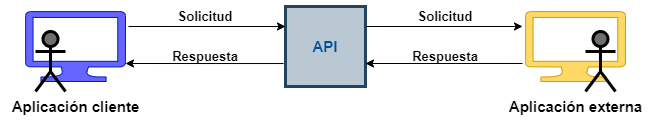
\includegraphics[scale=0.6]{img/APIs.png}
    \caption{Conceptos teóricos - APIs}
    \label{Conceptos teóricos - APIs}
\end{figure}

Podemos encontrar 4 tipos de APIs diferentes:
\begin{enumerate}
    \item APIs públicas: son APIs que pueden ser utilizadas libremente sin tener apenas restricciones.
    \item APIs privadas: son APIs que solo podrán usarse dentro de una propia organización.
    \item APIs de socios: son APIs utilizadas exclusivamente por los socios que competen una alianza comercial.
    \item APIs compuestas: son aquellas que hacen uso de otras APIs de servicio.
\end{enumerate}

\subsection{API de Twitter}

La API de Twitter \cite{apiTwitter} se utiliza para obtener los datos de los tweets según una búsqueda específica, en este caso, Bienes de Interés Cultural del Camino de Santiago Francés en el tramo de Castilla y León (Figura 3.2). \\
\begin{figure}[h!]
    \centering
    
\includegraphics[scale=0.6]{img/APITwitter.png}
    \caption{Conceptos teóricos - API de Twitter}
    \label{Conceptos teóricos - API de Twitter}
\end{figure}

Dependiendo el uso que se le vaya a dar, Twitter ofrece varios niveles de acceso a ella.\\
Desde hace pocas fechas Twitter ha decidido cambiar la política de acceso a su API y los terminos y condiciones que se han utilizado en este proyecto (Figura 3.3).

\begin{enumerate}
    \item {Essential:} es la versión gratuita más básica. Se comenzó utilizando esta, pero más adelante se confirmó que sus recursos no eran suficientes para la realización del proyecto y se debía ascender el nivel de acceso. Permite recopilar 500.000 tweets al mes además de un proyecto por cuenta y acceso a la versión 2 de la API.\\ Sus limitaciones en la hora de la búsqueda son grandes. Lo más importante es que solo permite realizar búsquedas de los tweets más recientes
    
    \item {Elevated:} también es una versión gratuita, pero con más beneficios que la anterior. Permite recopilar 2 millones de tweets al mes y acceso a las versiones 1.1 y 2 de la API de Twitter.
    
    \item {Elevated+:} es un nivel que aún se está desarrollando y no está disponible actualmente. La ventaja que va a tener este nivel es que se podrán realizar hasta 10 millones de búsquedas de tweets al mes.
    
    \item {Academic Research:} este nivel es el utilizado en el proyecto. Para ello, como requisito principal se necesita que se demuestre que eres una persona del ámbito académico mediante un perfil que lo demuestre. No se puede utilizar para el uso comercial, solo para la realización de trabajos o tesis. Aumenta el número de tweets mensuales que pueden buscar a 10 millones y no hay  limitaciones en cuando a fechas de búsqueda, se puede buscar tweets desde la fecha de creación de Twitter.
    
\end{enumerate}
\begin{figure}[h!]
    \centering
    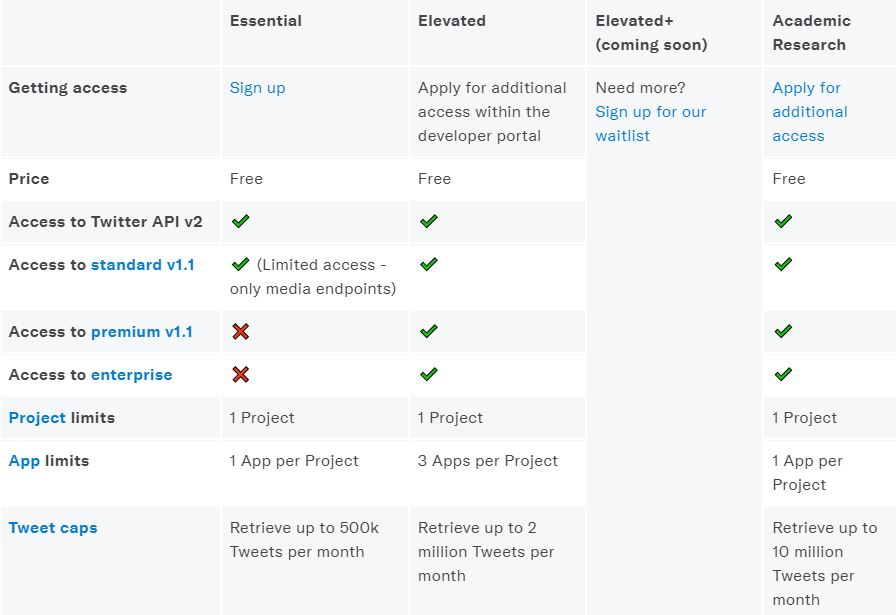
\includegraphics[scale=0.5]{img/nivelesDeAcceso.PNG}
    \caption{Diagrama de secuencia - Niveles de acceso de API Twitter}
    \label{Diagrama de secuencia - Niveles de acceso de API Twitter}
\end{figure}

\subsection{API Endpoint}
El API Endpoint o punto final de la API \cite{apiEndpoint}, es el punto exacto en el que se realiza la comunicación entre la aplicación del cliente y la API. En este punto se dan las solicitudes y respuestas de los implicados, a través de las operaciones GET, POST, DELETE y PATCH.

\subsection{URI}
El identificador uniforme de recursos o \textit{Uniform Resource Identifier} \cite{URI} se utiliza para identificar la información en internet e interactuar con el recurso que la almacena.
La URI está compuesta por cinco partes, dos de ellas obligatorias.
\begin{enumerate}
    \item \textbf{Esquema \textit{('scheme')}}: es una de las partes obligatorias que forman la URI, proporciona información sobre el protocolo que se ha utilizado.
    \item \textbf{Autoridad \textit{('authority')}}: es la parte que identifica el dominio.
    \item \textbf{Ruta \textit{('path')}}: es otra de las partes obligatorias, la cual define la ruta exacta al recurso.
    \item \textbf{Consulta \textit{('query')}}: es la parte define la acción de la consulta.
    \item \textbf{Fragmento \textit{('fragment')}}: se encarga de designar parte del principal recurso.
\end{enumerate}

\section{Series temporales}

Una serie temporal \cite{serieTemporal}es un conjunto de datos ordenados cronológicamente a lo largo de un tiempo determinado. 
Los datos de una serie temporal pueden ser de tres diferentes tipos:
\begin{enumerate}
    \item Datos de series temporales:\\
    Es el más comúnmente utilizado. Se muestran los valores de una variable en diferentes momentos cronológicos.
    \item Datos transversales:\\
    Se muestran en el mismo punto del tiempo los valores de una o más variables.
    \item Datos agrupados:\\
    Es la combinación de mostrar datos de series temporales y datos transversales.
\end{enumerate}
El análisis de las series temporales podemos realizarlo diferenciando cuatro características:
\begin{enumerate}
    \item Tendencia (T):\\
    Movimientos que realiza la serie de manera regular en un largo periodo de tiempo.
    \item Variaciones estacionales (E): \\
    Oscilaciones que realiza la serie temporal a corto plazo de manera regular.
    \item Variaciones cíclicas (C):\\
    Movimientos que realiza la serie temporal a corto plazo, donde el periodo y la amplitud pueden repetirse de manera regular.
    \item Variaciones irregulares o accidentales (A):\\
    Movimientos irregulares que se realizan en las series temporales de manera eventual.
\end{enumerate}
En este proyecto utilizan varios tipos de gráficos para plasmar diferentes tipos de series temporales, los gráficos a mostrar son los siguientes:
\begin{itemize}
    \item Gráfico de líneas:\cite{diagramaLineas}\\
    Es la represención de una o más variables a lo largo del tiempo (Figura 3.4). En este gráfico se podrán detectar repeticiones y si la variable sigue un patrón determinado o por lo contrario se comporta de manera irregular.
    \begin{figure}[h!]
        \centering
        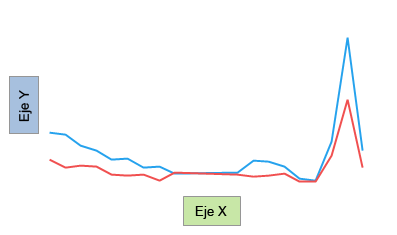
\includegraphics[scale=0.5]{img/GraficoLineas.PNG}
        \caption{Series temporales - Ejemplo de gráfico de lineas}\\
        \label{Series temporales - Ejemplo de gráfico de lineas}
    \end{figure}
    \item Gráfico circular:\cite{diagramaSectores}\\
    Es la manera de representar porcentualmente la frecuencia absoluta de la variable respecto al total durante un periodo de tiempo. \\
    Esta división se realiza sobre una circunferencia, seleccionando el ángulo del porcentaje de la variable a través de la fórmula de la Figura 3.5.
    \begin{figure}[h!]
        \centering
        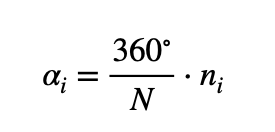
\includegraphics[scale=0.5]{img/FormulaDiagramasSectores.PNG}
        \caption{Series temporales - Fórmula del diagrama de sectores}
        \label{Series temporales - Fórmula del diagrama de sectores}
    \end{figure}
    Un ejemplo visual de cómo sería un gráfico circular se muestra en la Figura 3.6.
    \begin{figure}[h!]
        \centering
        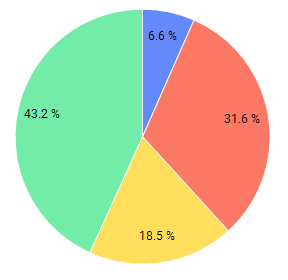
\includegraphics[scale=0.5]{img/GraficoCircular.PNG}
        \caption{Series temporales - Ejemplo de gráfico circular}
        \label{Series temporales - Ejemplo de gráfico circular}
    \end{figure}
    \item Gráfico de barras apiladas:\\
    Es la representación de comparar varias variables en el mismo punto a lo largo del tiempo (Figura 3.7). Estas se representan coloreando cada variable de un color y posicionandolas una encima de otra en el mismo punto en el tiempo hasta que la altura sume el total del valor de las variables en ese momento. Esta operación se repetirá tantas veces como días haya en el periodo de tiempo seleccionado.
    \begin{figure}[h!]
        \centering
        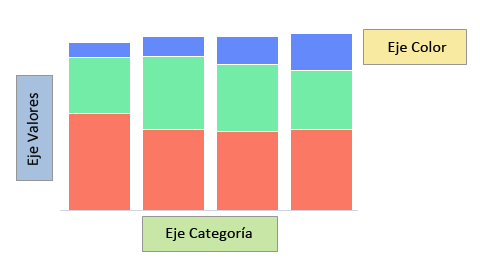
\includegraphics[scale=0.5]{img/GraficoBarrasApiladas.PNG}
        \caption{Series temporales - Ejemplo de gráfico de barras apiladas}
        \label{Series temporales - Ejemplo de gráfico de barras apiladas}
    \end{figure}
\end{itemize}
\section{Aplicación web}
Una aplicación web es un programa o servicio que se ejecuta en internet. Este programa guarda los datos y archivos en ella misma y no necesita que sea desargada en el equipo local.\\
Para realizar el desarrollo web de XacoMeterII se ha utilizado una base de datos, un framework, una plataforma de servicios en la nube y un protocolo HTTP.
\subsection{Base de datos}
Una base de datos \cite{BD} es un contenedor que puede almacenar una gran cantidad de información relacionada y ordenada, que más tarde puede ser buscada de manera mucho más sencilla.\\
Este almacen, además, puede ser manipulado por programas externos a través de unas credenciales.\\
Las bases de datos están formadas por tablas, cada una de ellas con la información que se desee, y además, esas tablas están organizadas por columnas, que son los parámetros diferenciados de la información con un tipo de dato asignado.
Cada uno de los registros de una tabla ordenadas por columnas, se llaman filas.
Las bases de datos se caracterizan por:
\begin{itemize}
    \item \textbf{Redundancia mínima:} la repetición de la información es la mínima, es decir, si un dato ya existe, si se utiliza en la base de datos, no se volverá a repetir.
    \item \textbf{Consistencia de los datos:} al repetir el menor número de información posible, se consigue que las actualizaciones o los borrados se realicen completamente, es decir, que todas las copias de la información sean consistentes.
    \item \textbf{Acceso concurrente por parte de múltiples usuarios:} el uso de una base de datos permite el acceso de varios usuarios al mismo tiempo, pudiendo mostrar toda la información necesaria simultáneamente.
    \item \textbf{Integridad de los datos:} una base de datos asegura poder recuperar los datos sin importar su antigüedad.
    \item \textbf{Consultas complejas optimizadas:} como la información de la base de datos está ordenada y organizada por parámetros, se puede buscar fácilmente y más rápido la información más compleja de encontrar.
    \item \textbf{Acceso a través de lenguajes de programación:} una base de datos permite acceder a ella a través de programas externos con varios lenguajes de programación.
\end{itemize}   
En este proyecto se utiliza una base de datos con lenguaje SQL \cite{sql}, que permite trabajar con los datos y las relaciones de los mismos.
Este lenguaje SQL permite las siguientes operaciones en una base de datos:
\begin{enumerate}
    \item \textbf{MOSTRAR:} a través de la operación 'SELECT'.
    \item \textbf{ACTUALIZAR:} a través de la operación 'UPDATE'.
    \item \textbf{INSERTAR:}  a través de la operación 'INSERT'.
    \item \textbf{BORRAR:} a través de la operación 'DELETE'.
\end{enumerate}
\subsection{Framework}
Un \textit{framework} \cite{framework} es una estructura base que sirve para el desarrollo de aplicaciones reutilizando herramientas y módulos. 
A través de los \textit{framework} se consigue reducir el tiempo de programación y los errores causados.
Dependiendo del lenguaje de programación se podrá elegir entre varios \textit{framework}. En este caso, XacoMeterII es un proyecto desarrollado en Python, por lo que se ha considerado que lo más conveniente es utilizar el \textit{framework} 'Flask'.

\subsection{Plataforma de servicios en la nube}
Una plataforma como servicio (PaaS) \cite{PaaS} es un conjunto de servicios integrados en la nube que permiten a los desarrolladores incluir todo lo necesario  para crear, ejecutar y gestionar aplicaciones.\\
En este proyecto se utilizará una plataforma de servicios en la nube (PaaS) llamada Heroku que permitirá el despliegue de la aplicación en la nube para que pueda ser utilizada por todos los usuarios de internet (Figura 3.8).
\begin{figure}[h!]
    \centering
    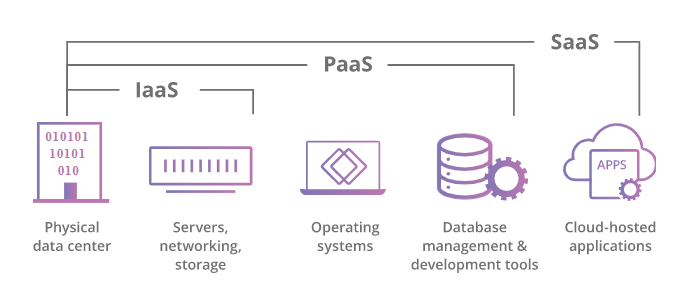
\includegraphics[scale=0.6]{img/PaaS.PNG}
    \caption{Conceptos teóricos - Plataforma de servicios en la nube}
    \label{Conceptos teóricos - Plataforma de servicios en la nube}
\end{figure}

\subsection{Protocolo HTTP}
El protocolo HTTP \textit{(Hypertext Transfer Protocol)} \cite{HTTP} es la manera que tienen de comunicarse un cliente con un servidor. El cliente solicita la información y el servidor se lo devuelve a modo de respuesta.
HTTP es un protocolo que no tiene estado: el cliente realiza una petición al servidor, este contesta y la transacción acaba, con lo que en la siguiente petición que pueda realizar el mismo cliente se deben proporcionar de nuevo todos los datos necesarios para que el servidor sirva correctamente la nueva petición.
\subsection{Sentiment analysis}
El proceso de Análisis de Sentimiento \cite{analisisSentimientos} consiste en la evaluación computacional de emociones, actitudes y opiniones presentes en un texto dado. Esta técnica es ampliamente utilizada por organizaciones para obtener la reacción de los clientes en relación a un producto o servicio en particular.\\
El Análisis de Sentimiento se realiza mediante el uso de tecnologías avanzadas de Inteligencia Artificial, incluyendo el Procesamiento del Lenguaje Natural, el Análisis de Texto y la Ciencia de Datos, con el objetivo de identificar, extraer y analizar información subjetiva presente en un texto. La herramienta clasifica un texto en tres categorías principales: positivo, negativo o neutral. 
\\En este caso específico, se utiliza una librería \cite{SentimentAnalysisSpanish} basada en Redes Neuronales para predecir el sentimiento de frases en español.\\
Sentiment-Analysis-Soanish ha entrenado una red neuronal convolucional con datos extraídos de diferentes páginas webs y redes sociales.

\capitulo{4}{Técnicas y herramientas}

\section{SCRUM}
Es un técnica de metodología ágil que se utiliza para la organización de un proyecto colaborativo en tareas.\\
Consiste en marcar una serie de periodos de tiempo y asignar tareas a cumplir con el objetivo de finalizar el proyecto de la manera más eficiente posible.
SCRUM se basa en llevar a cabo tres acciones claras:
\begin{enumerate}
    \item \textbf{Planificación:} se deben marcan las tareas a realizar, priorizando las más importantes.
    \item \textbf{Sprints:} durante el periodo de tiempo establecido, se deben realizar el mayor número de tareas marcadas en la planificación.
    \item \textbf{Burn Down:} una vez se finaliza el sprint, se deben visualizar los gráficos que muestren las tareas que se han realizado, con el tiempo que se ha invertido, y analizar si son los resultados que se esperaban, para corregirlos en el siguiente sprint.
\end{enumerate}

\subsection{GitHub}
Es una plataforma de código abierto que se utiliza para llevar el control de versiones. Permite almacenar información y código en un repositorio periódicamente para proteger los cambios realizados y que ninguno de ellos se extravíe. Existe una versión de escritorio y otra versión web, en este caso se ha utilizado la segunda opción.

\subsection{Zenhub}
Extensión para navegadores que complementa las utilidades que ofrece GitHub. Es una manera más visual de llevar a cabo la metodología SCRUM, ya que tiene una fácil asignación de tareas a través de un tablero Kanvan, y facilita crear los gráficos 'Burn Down' correspondientes a los sprints.

\section{Visual Code}
VS Code es un editor de código fuente de Microsoft que se ha utilizado para realizar el proyecto. Se ha elegido este editor porque facilita la depuración del programa durante su desarrollo, indica los errores de la sintaxis resaltándolos y permite una fácil conexión con el repositorio de GitHub para poder realizar los \textit{pull} y \textit{push} necesarios, así como la sincronización del código en cualquier momento.

\subsection{Python}
Lenguaje de programación flexible diseñado para ser fácil de leer, utilizado sobre todo para el desarrollo de sofware. Este lenguaje ha sido elegido para el desarrollo del proyecto debido a que ha sido uno de los lenguajes utilizados a lo largo de la carrera y, además, cuenta con varias librerias que facilitan la implementación de gráficos del programa.

\subsection{Flask}
Flask es un \textit{micro-framework} que permite integrar código Python para facilitar el desarrollo de aplicaciones web de forma sencilla y rápida. Es micro porque incluye solo las herramientas necesarias para el desarrollo del proyecto, pudiendo incluir \textit{plugins} si se considerase necesario.

\section{Microsoft Teams}
Aplicación de Microsoft 365 diseñada para permitir la comunicación entre usuarios, tanto en modo de chat como en el modo de llamada. Se ha utilizado para la comunicación con los tutores y realizar las reuniones pertinentes en cada sprint.

\section{Overleaf}
Es un editor de texto libre que permite escribir documentos con \LaTeX y a su vez compilarlos para ver el resultado final del mismo. Es una herramienta que permite la edición de los documentos con varios colaboradores y realizar comentarios que se utilizarán para la revisión de la documentación.
\subsection{\LaTeX}
Es un sistema de composición de textos que está pensado de tal manera que el autor debe centrarse más en el texto que en la forma. Sobre todo es utilizado para escribir fórmulas matemáticas, aunque puede ser utilizado en todos los ámbitos.

\section{Heroku}
Es una plataforma de servicios en la nube (PaaS) que se ha utilizado en este proyecto para desplegar la aplicación de manera sencilla. También se ha utilizado para subir la base de datos a la nube, utilizando Heroku PostgreSQL y que pueda accederse a ella desde la aplicación web y desde la aplicación local.

\section{PostgreSQL}
Sistema de base de datos relacional orientado a objetos de código abierto. Se ha decidido elegir PostgreSQL entre todas las opciones debido a que es sencilla de usar, se pueden visualizar los datos, es gratuita y Heroku permite su fácil despliegue.

\section{draw.io}
Aplicación web que permite el diseño de gráficos y diagramas para la explicación del proyecto en la documentación (diagramas de casos de uso, diagramas de secuencias, gráficos de APIs...)

\section{Librerías}
\subsection{Flask}
Librería utilizada para utilizar el framework Flask.
\subsection{Leaflet}
Librería utilizada para el desarrollo del mapa del inicio de la aplicación. Permite la implementación de mapas dinámicos con marcadores.
\subsection{Bootstrap}
Biblioteca de código abierto con la que se pueden diseñar aplicaciones web que permite la adptación de la misma al tamaño de la pantalla del dispositivo utilizado.
\subsection{Plotly}
Librería de Python que permite realizar gráficos dinámicos en dos dimensiones a partir de \textit{dataframes}.
\subsection{Pandas}
Librería de Python que permite realizar el análisis de datos, así como la manipulación de las mismas en formato de tablas o series.
\subsection{Werkzeug}
Librería utilizada para la seguridad de la aplicación, encriptando y desencriptando la contraseña del administrador utilizando el algoritmo \textit{PBKDF2 + SHA-256} para que ésta no sea accesible para usuarios no deseados.
\subsection{Psycopg2}
Librería utilizada para realizar la conexión con la base de datos PostgreSQL y poder realizar las operaciones deseadas en la misma.
\subsection{Dotenv}
Librería que se encarga de cargar las variables de entorno en el programa.
\subsection{Dateutil}
Librería de Python que tiene el fin de ampliar las funcionalidades de \textit{datetime}.
\subsection{Jinja2}
Es una de las librerías incluidas en Flask que sirve para generar plantillas HTML.
\subsection{Requests}
Biblioteca de Python que facilita el manejo de solicitudes HTTP. En este caso, se ha utilizado para realizar la comunicación con la API de Twitter y recibir la respuesta de la misma en forma de objeto \textit{response}.
\subsection{Sentiment-analysis-spanish}
Librería de Python que se ha utilizado para implementar el analisis de sentimientos, de tal manera que evalúa los textos de los tweets entre 0 y 1.
\begin{table}[ht!]
    \centering
    \begin{tabular}{c|c}
         \hline
         \textbf{Herramientas} & \textbf{Versión} \\\hline
         {Flask} &{2.2.2}  \\\hline
         {Leaflet} &{1.8.0} \\\hline
         {Bootstrap} &{12.16.1}\\\hline 
         {Plotly} &{3.6.3}\\\hline
         {Pandas} &{1.5.2} \\\hline 
         {Werkzeug} &{9.1.0}  \\\hline
         {psycopg2} &{2.9.5}\\\hline 
         {dotenv} &{0.21.0} \\\hline 
         {dateutil} &{2.8.2} \\\hline 
         {jinja2} &{3.1.2} \\\hline 
         {requests} &{2.28.2} \\\hline
         {sentiment-analysis-spanish}&{0.0.25}\\\hline
    \end{tabular}
    \caption{Técnicas y herramientas - Librerías}
    \label{Técnicas y herramientas - Librerías}
\end{table}
\capitulo{5}{Aspectos relevantes del desarrollo del proyecto}
En este apartado se pretende explicar las partes más significativas e importantes del desarrollo del proyecto, tanto su creación, diseño e interfaz gráfica, como las dificultades del mismo.

\section{Inicio del proyecto}
Tras hablar con José Ignacio y con Virginia de la posibilidad de realizar el TFG con ellos como tutores, comenzaron a pensar algún TFG que pudiesen ofrecerme. \\
En un inicio se valoró continuar con un trabajo anterior, desarrollado por un compañero en otro lenguaje, y ampliarlo de tal manera que se realizase un análisis de sentimientos y se implementase la nueva API de investigación de Twitter. Tras una reunión con los tutores, se decidió desarrollar desde cero una nueva aplicación, debido a que preferimos la opción de programarlo con un lenguaje aprendido durante los últimos años de carrera, para profundizar sobre él y facilitar su desarrollo. \\
\\\
Una vez iniciado el proyecto y habiendo tenido una primera reunión de toma de contacto, se presentó Silvia Díaz de la Fuente, investigadora predoctoral que se encuentra realizando una tesis sobre la gestión del patrimonio cultural en el Camino de Santiago Francés en Castilla y León. Con ella se va a realizar el proceso del desarrollo del proyecto ya que facilita la información más técnica del TFG.
\\\
\section{Primeros pasos}
Durante esta etapa se comienza investigando qué \textit{framework} utilizar. En un principio me decanté entre .NET y Django. La primera opción se descarta, ya que no es el mejor framework para el lenguaje Python, y la segunda opción resulta más atractiva para proyectos más grandes y robustos. Una opción parecida a Django pero más sencilla de utilizar es Flask, y dados los motivos explicados en el apartado anterior se decide decantarse por esta opción.
Además, se investigó sobre las herramientas que se iban a utilizar en un principio en el desarrollo de la aplicación y también sobre la API de Twitter, de la que se iba a extraer la información con la que trabajar durante el TFG.

\section{Formación}
Las herramientas y plataformas sobre las que se estudió su funcionamiento han sido:
\begin{itemize}
    \item \textbf{API de Twitter:} \\
    El proyecto de TFG XacoMeterII se enfoca en la implementación de la API de Twitter para la extracción de datos relevantes. Antes de iniciar la implementación, se llevó a cabo un análisis y evaluación de la funcionalidad de la API de Twitter y las distintas alternativas disponibles para su integración.\\
    Este análisis incluyó la identificación de los recursos y métodos de la API de Twitter que serían necesarios para el proyecto, así como la evaluación de las restricciones y limitaciones de la API. También se consideraron las diferentes alternativas de integración, bibliotecas y las técnicas de autenticación.\\ 
    Además, se realizó una evaluación de la documentación y los recursos de apoyo disponibles, incluída la comunidad de desarrolladores. Al final se decidió realizar la conexión a través de la librería \textit{'requests'}, ya que es una biblioteca más genérica y versátil que se puede utilizar para hacer peticiones HTTP a cualquier servicio web, no solo a la API de Twitter, y así entender bien el funcionamiento de conexión con las APIs.\\
    \item \textbf{Flask, .NET, Django:}\\
    Se eligió utilizar Flask como \textit{framework} para la creación de la aplicación debido a su facilidad de uso e instalación. Flask permite crear un servidor en Python de manera rápida y eficiente, y es una buena opción para proyectos de tamaño mediano y pequeño. Además, su diseño favorece el patrón de arquitectura MVC, lo que facilita la separación clara entre el modelo, la vista y el controlador.\\
    Aunque también se consideró la opción de utilizar Django o .NET, se decidió optar por Flask debido a su enfoque en proyectos más pequeños y simplificados. Django y .NET son marcos de trabajo más completos y orientados a proyectos de mayor escala. En este caso, Flask se adaptaba perfectamente a las necesidades y requerimientos de la aplicación.
    \item \textbf{Matplotlib, Plotly:}\\
    En un primer momento, se decidió utilizar la librería \textit{'Matplotlib'} para la generación de gráficos en el proyecto XacoMeterII, debido a la familiaridad con la misma, adquirida a través del uso previo en diversas asignaturas del grado.\\ 
    Sin embargo, con el avance del proyecto se consideró que sería más adecuado utilizar la librería \textit{'Plotly'} para la generación de gráficos interactivos.\\
    Para ello, se realizó una investigación en la página web de Plotly para adquirir conocimiento sobre su funcionamiento y características. Plotly es una librería de gráficos interactivos y visualización de datos que permite crear gráficos atractivos y fácilmente interactuables, y es ampliamente utilizada en aplicaciones web y móviles.\\
    Al usar Plotly, se pudo mejorar la representación visual de los resultados obtenidos a través de la extracción de datos de la API de Twitter.

\end{itemize}
\section{Metodología}
La metodología adoptada en este proyecto es SCRUM, aprendida en la asignatura de Gestión de Proyectos. Se basa en la aplicación de la metodología ágil para la gestión del proyecto, dividiendo el tiempo en periodos iterativos conocidos como \textit{"Sprints"}, en los cuales se establecen los objetivos y se realiza una estimación del coste temporal utilizando Story Points. 
\\La herramienta Zenhub ha sido utilizada para este proceso, ya que proporciona una plataforma de trabajo visual donde se puede interactuar con las tareas de manera sencilla y generar los gráficos.\\

En cuanto a las reuniones, se han realizado aproximadamente cada dos semanas. En ellas se llevaba a cabo una revisión del trabajo realizado, evaluando el progreso e identificando los objetivos cumplidos, la retrospectiva de dicho Sprint, exponiendo los problemas encontrados e identificando los aspectos a mejorar y la planificación del siguiente para establecer los objetivos a alcanzar y estimar el trabajo requerido para cada tarea.


\section{Desarrollo del proyecto}
\subsection{Implementación de la API de Twitter}
Una vez investigadas las herramientas que se iban a  poner en uso, se pudo comenzar a implementar la API de Twitter. En un inicio se realizó la conexión con la API a través de la herramienta \textit{Tweepy} y probando con un acceso \textit{'Essential'}, el cual solo permitía recoger los tweets más recientes.\\
Una vez implementado con el acceso más básico, se organizó una reunión con los tutores, y Virginia, al tener una página web en la que se la reconocía como docente de la Universidad de Burgos, pudo solicitar el acceso como investigadora a la API. Para ello contactó a través de la plataforma de \textit{Twitter developers} con Twitter y consiguió obtener las credenciales necesarias para realizar la conexión.\\
Se intentó durante un sprint conectar con la API a través de los nuevos datos de acceso, pero no hubo resultado.\\
Este paso causó varios problemas, ya que aplicando varios métodos de conexión no se obtuvo la respuesta esperada de la API de Twitter. Esto ralentizó mucho el proceso del desarrollo del proyecto, por lo que se decidió realizar otra reunión y tras revisar bien todos los pasos, se descubrió que no se había activado correctamente el nuevo acceso. \\
Al final se implementó la conexión con la API de Twitter mediante el uso de la biblioteca \textit{'requests'} en Python. Se definen varias funciones en el fichero \texttt{Code/FuncionPrincipal\_XacoMeterII.py} encargadas de autentificarse, acceder a los encabezados, realizar la solicitud a la API y conectarse a la API para obtener los datos deseados.\\
\begin{itemize}
    \item La función \textbf{auth} se encarga de devolver el \textit{token} de autenticación, el cual es un valor almacenado en una variable de entorno. La función 'accederEncabezados' recibe el token y devuelve los encabezados necesarios para la solicitud a la API, que incluyen la autorización.
    \item La función \textbf{solicitudURL} recibe como argumentos la palabra clave a buscar, la fecha de inicio y la fecha de fin, y devuelve la URL de \textit{endpoint} y los parámetros de búsqueda para la solicitud.
    \item La función \textbf{conexionEndpoint} es la encargada de realizar la solicitud a la API y devolver la respuesta en formato JSON. Recibe la URL del \textit{endpoint}, los encabezados y los parámetros de búsqueda.
    \item Finalmente, la función \textbf{funcionPrincipal} define las variables y hace las llamadas a las funciones anteriores para obtener la información deseada. Devuelve un diccionario con los tweets obtenidos de la API de Twitter para poder incluirlos en la base de datos PostgreSQL de manera sencilla a través de una query.
\end{itemize}

La API de Twitter con acceso de investigador académico tiene unas restricciones que han hecho que el proceso sea mucho más lento de lo esperado en un principio (Figura 5.1)\\
\begin{figure}[h!]
    \centering
    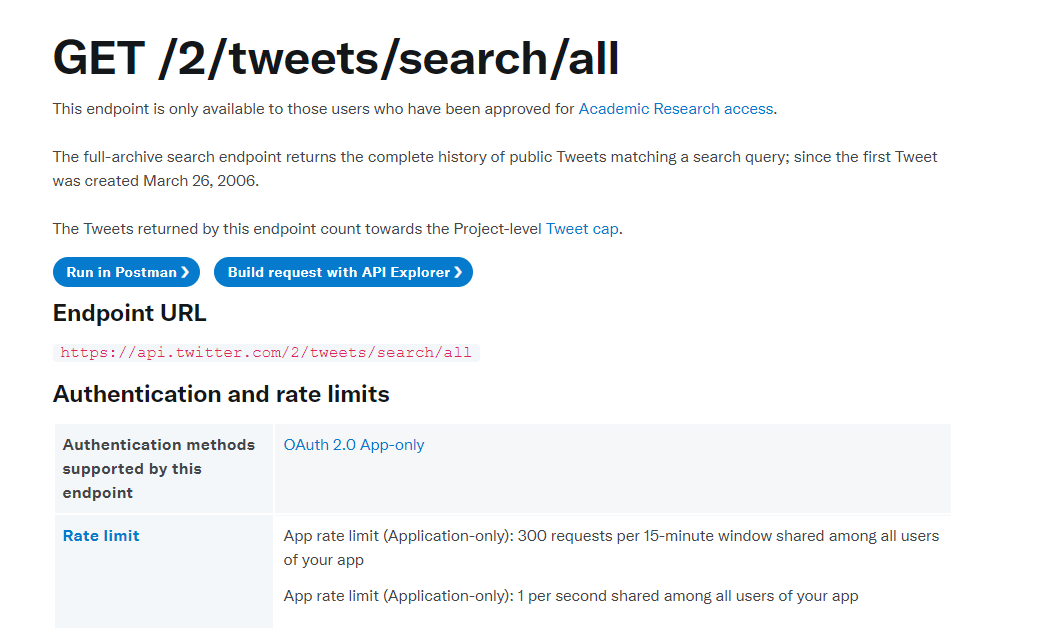
\includegraphics[scale=0.5]{img/SearchAll.png} \\
    \caption{Aspectos relevantes - API Twitter}
    \label{Aspectos relevantes - API Twitter}
\end{figure}
\begin{enumerate}
    \item Solo se pueden realizar 300 consultas cada 15 minutos.
    \item Cada petición debe durar mínimo 1 segundo.
    \item En cada petición se pueden obtener máximo 150 tweets.
\end{enumerate}
Así se ha tenido que configurar la parte del administrador, quien recopila los datos, de tal manera que introduzca unos parámetros para la búsqueda, para que en un futuro no se deba cambiar el código en el caso de que cambien las restricciones y con ellos, realizar paradas de tiempo (Figura 5.2).\\
\begin{figure}[h!]
    \centering
    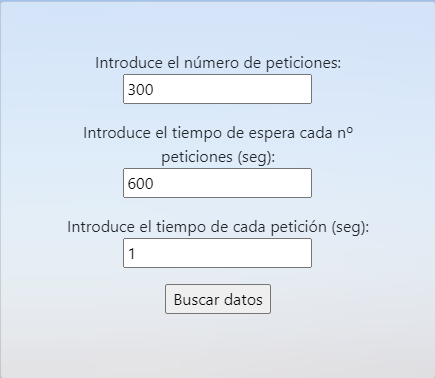
\includegraphics[scale=0.5]{img/parametrosBusqueda.png} \\
    \caption{Aspectos relevantes - Parámetros administrador}
    \label{Aspectos relevantes - Parametros administrador}
\end{figure}
Como en cada petición solo se pueden obtener 150 tweets y hay BICs que obtienen bastantes datos al día, se ha decidido realizar una petición al día por cada BIC, lo que quiere decir, que mínimo se van a realizar 130 peticiones para recopilar datos de un día completo de todos los BICs.\\
Actualmente solo se podrán realizar máximo 300 consultas cada 15 minutos y cada una de ellas debe durar mínimo 1 segundo. Además, se podrá calcular el tiempo de espera entre las consultas especificadas en el primer parámetro y las siguientes consultas. Twitter ha definido que se podrán realizar máximo 300 consultas cada 15 minutos, por lo que se recomienda esperar 10 minutos, es decir, 600 segundos:\\
    $$ 15\hspace{0.5em}minutos\times60\frac{\text{segundos}}{\text{minuto}}=900\hspace{0.5em}segundos $$
    $$ 300\hspace{0.5em}peticiones\times1\frac{\text{segundo}}{\text{petición}}=300\hspace{0.5em}segundos $$
    $$ 900\hspace{0.5em}segundos\hspace{0.5em}-\hspace{0.5em} 300\hspace{0.5em}segundos\hspace{0.5em}=\hspace{0.5em}600\hspace{0.5em}segundos$$
Twitter ha anunciado recientemente que se está realizando un cambio en su política de acceso a su plataforma a partir del 9 de Febrero. En lugar de ofrecer acceso gratuito a su API, Twitter implementará un nivel con una tarifa básica para su acceso (Figura 5.3).\\
\begin{figure}[h!]
    \centering
    
\includegraphics[scale=0.5]{img/TwitterDev.png} \\
    \caption{Aspectos relevantes - Comunicado Twitter}
    \label{Aspectos relevantes - Comunicado Twitter}
\end{figure}
\subsection{Creación y conexión de la base de datos}
Primeramente, para probar el funcionamiento de la API, se creaba un csv en el que se almacenaban los datos y así se podía comprobar si verdaderamente estaba realizando las operaciones correctamente.\\ Una vez comprobado, se procedió a crear una base de datos para almacenar la información. \\
Se quería utilizar una base de datos en la nube, pero tras buscar entre varias opciones, o no tenían gran capacidad de almacenamiento, o no eran en la nube. Debido a estas dificultades, se decidió utilizar una base de datos que pudiese ser desplegada en la nube, por lo que nos decantamos por PostgreSQL.
En un inicio, se comenzaron creando dos tablas en la base de datos local, y que, a partir del csv temporal se introdujesen los datos en PostgreSQL. Estas dos tablas eran la tabla en la que se almacenasen los nombres de los patrimonios con un id identificativo y la tabla en la que se guardase toda la información obtenida de la API de Twitter, con una clave foránea del id del nombre del BIC que se conectase con la tabla de nombres.

\subsection{Desarrollo de la parte visual del proyecto}
Una vez se tuvo la conexión con la API y la base de datos montada, se decidió crear una interfaz gráfica muy sencilla para ver algún resultado. Lo único que se desarrolló fue una nube de palabras donde se destacasen las palabras clave de los textos y un inicio con el nombre del proyecto. 
A lo largo del proyecto se fueron decidiendo aspectos que se querían incluir en la interfaz.
A partir de aquí, se fue ampliando de tal manera que:
\begin{enumerate}
    \item Primero, se decidió poner varios botones que permitiesen manejar la API, pidiéndola los tweets de todos los BICs marcando solo una fecha desde la que se requerían los datos. Esta acción, si la fecha era posterior a la primera fecha de la base de datos, borraba todos los registros entre las dos de la base de datos.
    \item La interfaz se fue mejorando y se incluyó que, además de crearlos desde una fecha, se pudiesen actualizar desde la última fecha registrada en la base de datos hasta la fecha actual.
    \item Al ver que la extracción de datos era bastante pesada, se decidió incluir un parámetro en la base de datos, booleano, en el que se marcase si el registro estaba eliminado o no, evitando de esta manera borrar registros de la base de datos y aumentando el rendimiento de extracción de datos de la API, ya que se no se tendrían que volver a solicitar dicha información.
    \item Estas acciones de actualizar o crear registros en la base de datos es un factor que pensamos que no todo el mundo debe controlar, por lo que decidimos que la mejor opción sería que solo un administrador con un usuario y una contraseña pudiese acceder, mientras que los usuarios generales solo pudiesen ver las estadísticas de los datos.
    \item Para que el inicio de sesión del usuario fuese seguro, primero se insertó en la base de datos un registro con el nombre de usuario y una contraseña encriptada.\\
    El usuario que desee realizar acciones de administrador deberá introducir un usuario y una contraseña, y si el nombre de usuario se encuentra en la base de datos, entonces se encripta la contraseña insertada y se compara con la de la base de datos. Solo en este caso se podrá acceder como administrador.
\end{enumerate}
\subsection{Creación de mapa didáctico}
Para las páginas accesibles para todos los usuarios, se comentó crear un mapa geográfico con los BICs ubicados en él. Primero se probó poniendo de fondo una imagen de un mapa y, sobre él, situar botones en los lugares más convenientes por pixeles. \\
Al ver que esa opción no estaba dando el resultado esperado, se pensó en implementar la API de Google, pero es una API de pago y se buscaron otras alternativas. \\
Al final, se encontró la herrmienta de \textit{'leaflet'}, que mediante coordenadas, permite insertar un mapa con un punto medio de visión y sobre él, se posicionan los marcadores por las coordenadas latitud y altitud situando todos los BICs a partir de datos almacenados en un csv (Figura 5.4).\\
También se pensó que, al haber 130 BICs, el mapa queda muy condensado, por lo que se podrían poner solo las localidades, y al hacer click sobre ellas, se redireccionase a una página con las imágenes de los patrimonios.\\
Silvia realizó una recopilación de imágenes relevantes para su investigación. Sin embargo, no disponía de las imágenes de todos los BICs y, debido a restricciones de derechos de autor si eran sacadas de internet se optó por no insertar imágenes.\\
Al final, se ubicaron todos los BICs en el mapa. 
Además, se implementó una funcionalidad de \textit{'popups'} en cada uno de los BICs, que incluía un enlace a la página donde se generan estadísticas específicas para cada bien. Se utilizó la función de hacer \textit{'hover'}, es decir, pasar el ratón, sobre el icono para mostrar el nombre del BIC sin necesidad de pulsar en cada uno de ellos.
\begin{figure}[h!]
    \centering
    \includegraphics[scale=0.3]{img/mapa.png} \\
    \caption{Aspectos relevantes - Mapa}
    \label{Aspectos relevantes - Mapa}
\end{figure}
\subsection{Creación de página de estadísticas}
Para la creación de la página de estadísticas, en un principio, se iba a insertar solo un gráfico temporal que mostrase el número de tweets publicados del BIC elegido en el mapa de todas las fechas almacenadas en la base de datos. \\
Estos gráficos se realizaron con la herramienta de \textit{'Matplotlib'} que facilita bastante la inserción de gráficos con el lenguaje Python.\\
Al tener bastantes datos en PostgreSQL, se decidió también crear otro tipo de gráficos. 
\begin{itemize}
    \item El gráfico temporal ya creado.
    \item Un gráfico circular que comparase los tweets del BIC seleccionado durante esa fecha respecto al total de tweets almacenados en la base de datos de todos los bienes históricos.
    \item Por último, resultaba interesante que al haber guardado las métricas públicas de los tweets, se pudiese realizar un gráfico de barras apiladas comparando los \textit{likes, retweets y replies} que se obtuvieron del BIC entre las fechas seleccionadas.
\end{itemize} 
Para poder realizar una búsqueda más específica, se añadió la opción de poder cambiar el rango de fechas para realizar las estadísticas, con dos calendarios en los que se puede seleccionar la fecha de inicio y de fin, siendo la primera fecha menor que la segunda.\\
En el caso de que no se inserte ninguna fecha, se utilizarán por defecto la primera fecha almacenada en la base de datos y la última.
\subsection{Despliegue con  Heroku}
Una vez se tuvo la aplicación montada en local, se comenzó el proceso de despliegue en Heroku. Para que la base de datos pueda ser accesible, también se añadió en Heroku un \textit{add-on} de Heroku-PostreSQL para desplegar la base de datos en la nube.\\
Para desplegar la base de datos se obtuvieron las credenciales de Heroku-PostgreSQL y se cambiaron en la aplicación por las que anteriormente habíamos insertado de la base de datos local. Además se configuró en PostgreSQL la nueva base de datos, transladando los datos anteriormente recuperados a través de un 'backup'.
\section{Mejoras}
Una vez completadas las funcionalidades básicas de la aplicación, se decidió mejorar la experiencia de usuario agregando una barra de navegación con una función de búsqueda para facilitar la interacción (Figura 5.5).\\

\begin{figure}[h!]
    \centering
    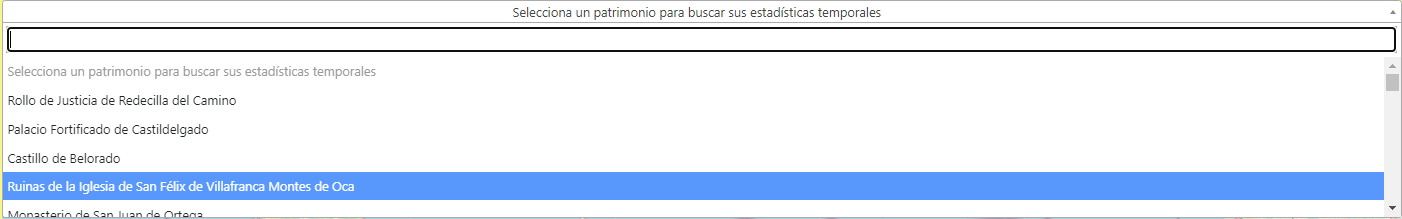
\includegraphics[scale=0.3]{img/busqueda.png} \\
    \caption{Aspectos relevantes - Barra navegadora}
    \label{Aspectos relevantes - Barra navegadora}
\end{figure}
Para garantizar la resolución de posibles errores en la aplicación, se implementaron mensajes de error para que los usuarios y el administrador puedan identificar y solucionar fácilmente los problemas (Figura 5.6).\\
\begin{figure}[h!]
    \centering
    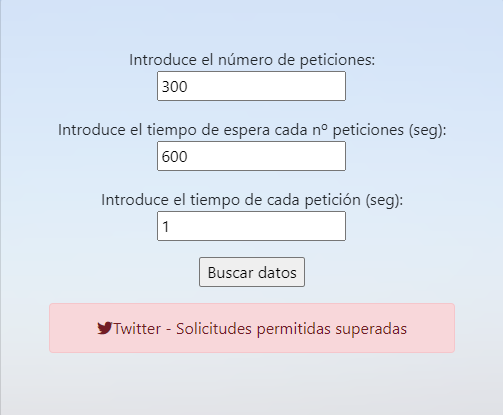
\includegraphics[scale=0.55]{img/errores.png} 
    \caption{Aspectos relevantes - Notificación de errores}
    \label{Aspectos relevantes - Notificación de errores}
\end{figure}
Para mejorar la presentación de los datos en la página de estadísticas, se implementó la librería \textit{'Plotly'} para generar gráficos interactivos, permitiendo al usuario realizar más acciones además de la visualización, como mover los gráficos.\\
Además, se incluyó una página de estadísticas temporales global con un gráfico de comparación de todos los BICs en un rango de fechas seleccionado (Figura 5.7).\\
\begin{figure}[h!]
    \centering
    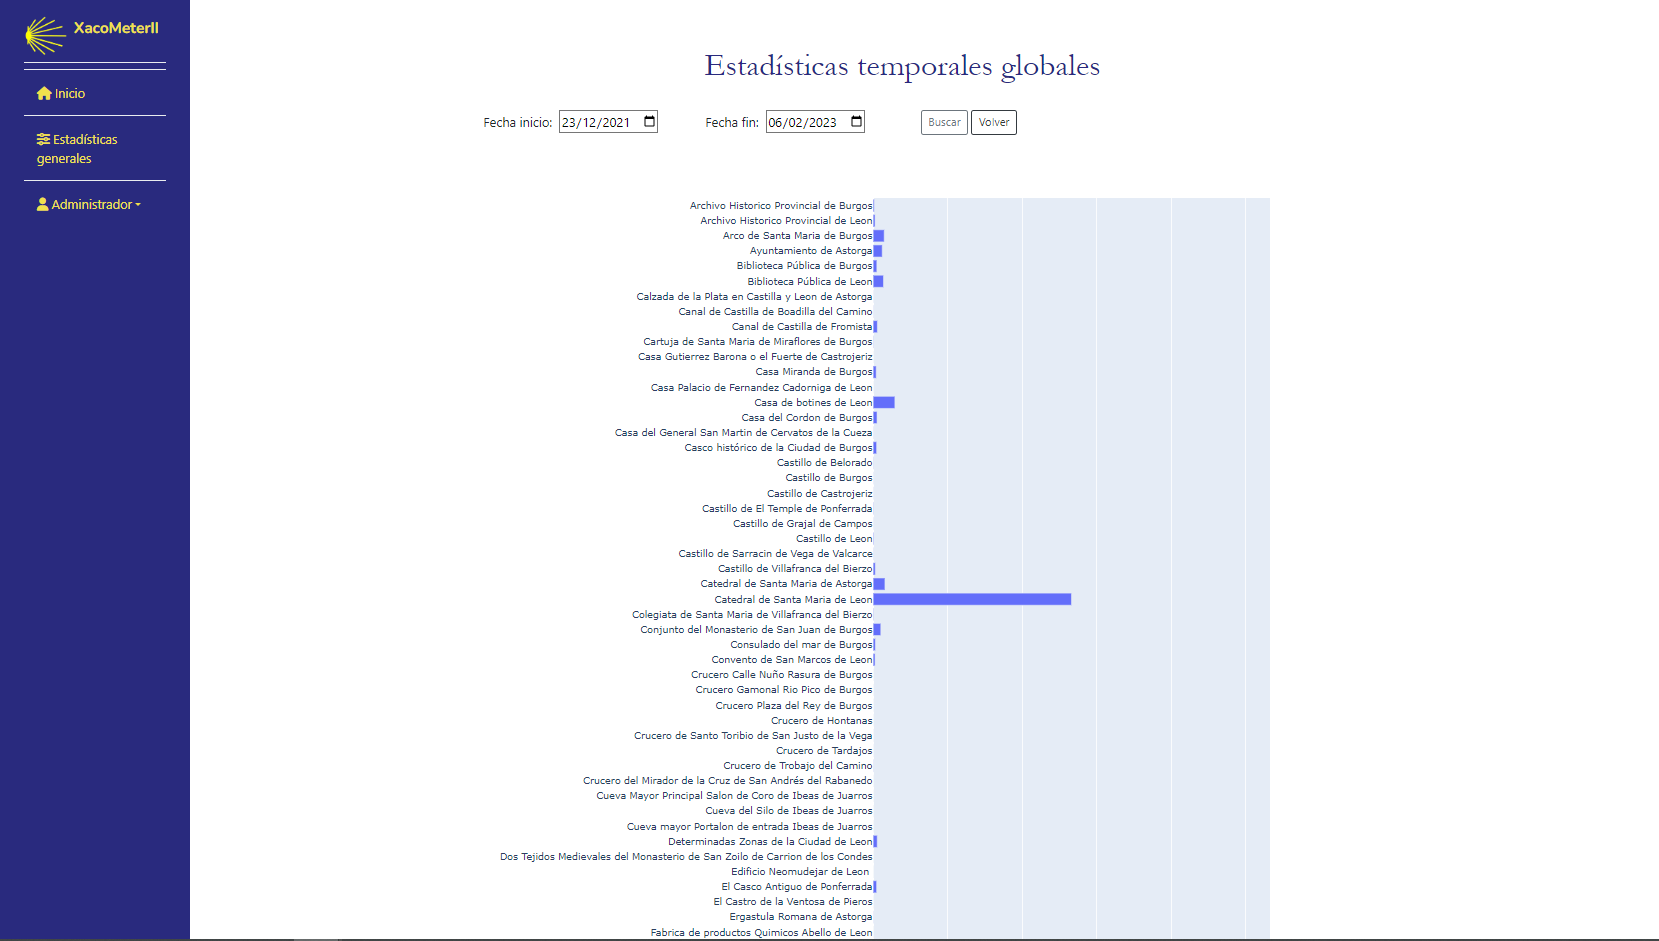
\includegraphics[scale=0.3]{img/EstadisticasGenerales.png}
    \caption{Aspectos relevantes - Estadísticas generales}
    \label{Aspectos relevantes - Estadísticas generales}
\end{figure}
\\
Por último, se agregó un análisis de sentimientos, que evaluará el sentimiento (positivo, neutral o negativo) en un número decimal entre 0 y 1, y se mostrará en un gráfico semicircular en la página de estadísticas del BIC. Se realizará una media de los sentimientos entre las fechas indicadas por el usuario (Figura 5.8).\\
\begin{figure}[h!]
    \centering
    \includegraphics[scale=0.3]{img/mejoras.png} \\
    \caption{Aspectos relevantes - Estadísticas mejoradas}
    \label{Aspectos relevantes - Estadísticas mejoradas}
\end{figure}
\capitulo{6}{Trabajos relacionados}

\section{XacoMeter - App}
Es una aplicación web creada por el alumno Daniel Tendero de la Universidad de Uurgos como su trabajo de fin de carrera. La aplicación monitoriza el Camino de Santiago a partir de información de tweets, y obtiene estadísticas relevantes del mismo.
\begin{itemize}
    \item Recupera los datos de \textit{hashtags} de Twitter relacionados con el Camino de Santiago.
    \item Permite que los usuarios se registren e inicien sesión.
    \item Obtiene los últimos tweets de los \textit{hashtags} seleccionados.
    \item Realiza un análisis de sentimiento de los tweets. Aunque como se desarrolló en JavaScript, la evaluación de sentimientos es muy primitiva basándose en contar palabras positivas y negativas.
    \item Permite que los usuarios administradores modifiquen los hashtags y las palabras clave del sistema.
    \item Soporta varios idiomas.
\end{itemize}







\capitulo{7}{Conclusiones y Líneas de trabajo futuras}


\subsection{Conclusiones}

Después de varios meses de intensa dedicación y esfuerzo en el proyecto XacoMeterII, se puede afirmar con certeza que se ha experimentado un significativo crecimiento y desarrollo tanto a nivel técnico como personal. Durante este proceso, se han adquirido habilidades y conocimientos valiosos en el campo de la programación, que han permitido mejorar las capacidades y competencias en esta área. Además, el trabajo en equipo junto con mis tutores y la resolución de desafíos han fomentado un crecimiento personal y profesional. En definitiva, el proyecto XacoMeterII ha sido una experiencia enriquecedora y formativa a nivel individual.\\

El proyecto finalmente ha cumplido con todos los objetivos marcados en un principio, añadiendo además nuevas funcionalidades que hacen a XacoMeterII una aplicación más atractiva visualmente y que permite a los usuarios interactuar con ella en cualquier dispositivo con acceso a Internet.\\

En un principio, XacoMeterII iba a ser una aplicación web que utilizase la API de Twitter para obtener los datos de una serie de bienes histórico-artísticos y mostrarlos con un gráfico al usuario.\\
Según fue avanzando el proyecto se fueron añadiendo nuevas funcionalidades, comenzando por tener un inicio de sesión para separar las funcionalidades de la aplicación y permitir solo al administrador realizar acciones en la base de datos. Se continúo con la implementación de un mapa didáctico para la búsqueda de BICs y, además de mejorar todas las ideas iniciales, se acabó ampliando el proyecto para realizar un análisis de sentimientos de cada uno de los tweets.\\

Personalmente, he de decir que he aprendido mucho sobre el manejo de las APIs, nunca había desarrollado ni había investigado sobre su uso y me ha hecho salir de mi zona de confort y poder ampliar conocimientos. He podido mejorar y practicar con conceptos ya aprendidos en la carrera, como la metodología SCRUM, que gracias a la cual he conseguido llevar un control del proyecto y una buena organización o como las bases de datos, pudiendo gestionar todos los datos y organizarlos de la mejor manera para este proyecto, y también el lenguaje Python, ya que es un lenguaje que personalmente me gusta mucho y he podido aprender más sobre él. \\
También he podido aprender a desarrollar una aplicación web desde cero, cosa que nunca había hecho, poder entender de manera práctica el modelo-vista controlador, ya que se había estudiado de manera teórica pero no se había llevado a la práctica y, aunque pueden quedar cosas que mejorar, se ha conseguido realizar todas las conexiones de manera exitosa y terminar el proyecto de manera satisfactoria.\\

Después de lo comentado, en mi opinión mi curva de mi aprendizaje ha sido buena aun con las dificultades encontradas en el proyecto.

\subsection{Líneas de trabajo futuras}
\begin{itemize}
    \item Poder crear cuentas para los usuarios y que puedan guardar sus historiales de búsquedas.
    \item Ampliar el análisis de sentimientos y evaluar la precisión de los resultados.
    \item Realizar un proceso en segundo plano para que en el caso de querer actualizar o crear la base de datos en la aplicación desplegada no termine con on \textit{'Timeout'}.
    \item Dar la opción de cambiar el idioma de la aplicación.
\end{itemize}

 



\bibliographystyle{plain}
\bibliography{bibliografia}

\end{document}
